\documentclass[10pt,a4paper]{article}
\usepackage[utf8]{inputenc}
\usepackage{amsmath}
\usepackage{amsfonts}
\usepackage{amssymb}
\usepackage{graphicx}
\usepackage{float}
\usepackage{listings}
\usepackage{color}

\definecolor{dkgreen}{rgb}{0,0.6,0}
\definecolor{gray}{rgb}{0.5,0.5,0.5}
\definecolor{mauve}{rgb}{0.58,0,0.82}

\lstset{frame=tb,
  language=Python,
  aboveskip=3mm,
  belowskip=3mm,
  showstringspaces=false,
  columns=flexible,
  basicstyle={\small\ttfamily},
  numbers=none,
  numberstyle=\tiny\color{gray},
  keywordstyle=\color{blue},
  commentstyle=\color{dkgreen},
  stringstyle=\color{mauve},
  breaklines=true,
  breakatwhitespace=true,
  tabsize=3
}

\graphicspath{ {figures/} }

\author{Kevin Thompson}
\title{Filtering Spam with Multinomial Naive Bayes}
\begin{document}
\maketitle



\section{Introduction}
Spam irritates end users and poses a security risk for companies. Employees who do not realize they are interacting with spam may, for example, mindlessly click on attachments within the email and infect their computer with ransomware or other types of malware. An automated solution that filters out spam is therefore a necessary and potentially pro-social solution. Since we are only concerned with classifying messages as "spam or "not spam", the spam filtering problem can be reduced to a binary classification problem, which is one of the most well-understood machine learning problems in artifical intelligence.

I solve this problem by implementing an email parsing program that efficiently converts the the great diversity of email files into a uniform data representation and then fit a multinomial naive bayes algorithm using the provided text data.

\section{Methodology}
The solution is comprised of the following parts:
\begin{enumerate}
\item An email parsing engine dynamically assigns parsing strategies to different email formats in an efficient manner. The engine provides a vocabulary and a pandas dataframe.
\item A count vectorizer from the Scikit-learn Package.
\item A grid search crossvalidation object that searches for the optimal smoothing hyperparameter ($\alpha$) in the family of Multinomial Naive Bayes models.
\item The model with the highest f1-score produced by the crossvalidation object is evaluated on test data to assess its performance.
\end{enumerate}

\subsection{Email Parsing Engine}

The parsing engine takes a directory of email files and dynamically assigns a parsing strategy to each file at runtime. The files are parsed into an intermediate representation defined by the class "Email" that is stored in an "EmailDatabase" object. The Engine then takes the email objects and converts them into a vocabulary and a dataframe. The vocabulary is bi-directional dictionary that serves as an encoder and decoder for situations in which an alternative encoder is not available. For the naive bayes model used in this project, the scikit-learn "CountVectorizer" is used instead since bayes's rule relies on counts in the discrete setting.

The Universal Modeling Language (UML) class diagram representig the email preprocessing program is shown in Figure \ref{emailUML} and the code that implements this program can be found in Appendix A.


\begin{figure}
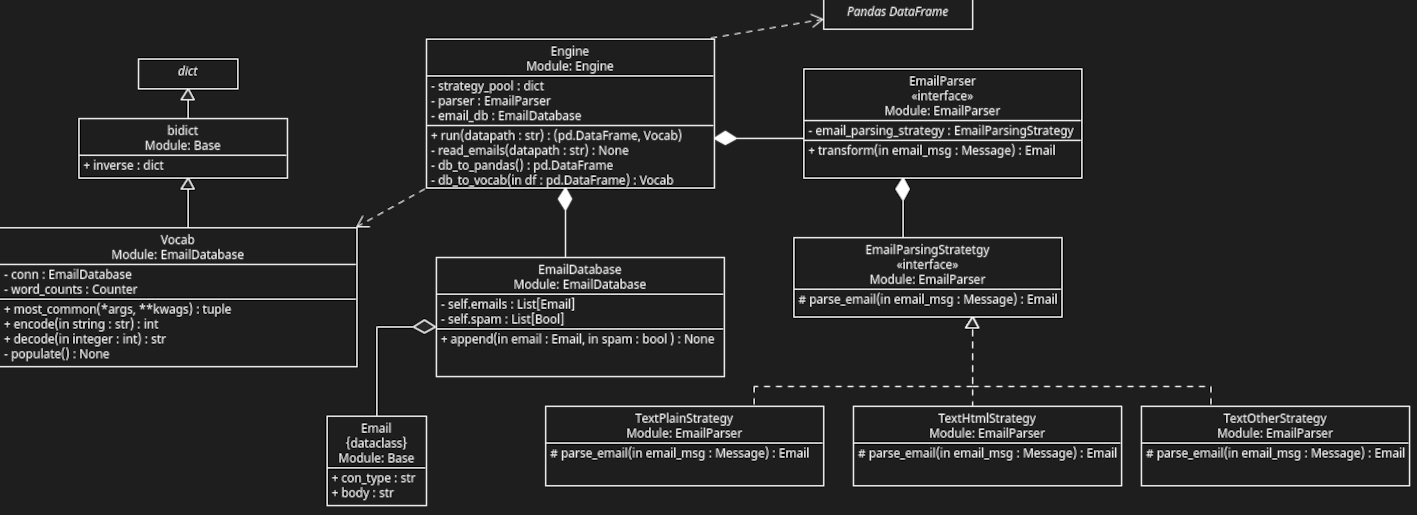
\includegraphics{umlclassdiagscaled.png}
\caption{UML class diagram representing the email preprocessing program's structure. The entirety of the logic is encapsulated by the Engine class.}
\label{emailUML}
\end{figure}

\subsection{Multinomial Naive Bayes}

Define the set of class labels to be $\mathcal{G} := \{\text{Spam}, \ \text{Not Spam}\}$.
Let $y \in \{0,1\}^{n}$ be a binary-valued n-vector generated by target label encoding function $\mathcal{E}: \mathcal{G}^{n} \longrightarrow \{0,1\}^{n}$ defined by
\[
y_{i} = 
	\begin{cases}
	1 & \text{if $g_{i} = \text{Spam}$,} \\
	0 & \text{if $g_{i} = \text{Not Spam}$,}
	\end{cases}
\]
where $i \in \{1, \ 2, \ ... \ , \ n\}$, and $X \in \mathbb{R}^{n \times q}$ be an n-by-q matrix of numerically-encoded tokens.

For this use case, it is assumed that every document $d$ consists of a collection of tokens \textbf{t} with $t_{k}$ denoting the kth token in the vocabulary of words.

The probability of a document d being in a class g is computed as

\begin{equation} \label{probabilitymodel}
P(g|d) \propto P(g) \prod_{1 \leq k \leq n_{d}}P(t_{k}|g),
\end{equation}

where $n_{d}$ denotes the number of tokens in document d.

The decision rule for classifying document d, $g_{map}$, is determined by the maximum a posteriori (MAP) class: 

\begin{equation}
g_{map} = arg max_{g \in \mathcal{G}}\hat{P}(g|d) = arg max_{g \in \mathcal{G}}\hat{P}(g)\prod_{1\leq k \leq n_{d}}\hat{P}(t_{k}|g),
\end{equation}

where $\hat{P}$ denotes the empirical probability. 

Because the probability of an event is definitionally non-negative and logarithmic functions are monotonic, Equation (\ref{probabilitymodel}) can be simplified to

\begin{equation}
\log{P(g|d)} \propto \log{P(g)} + \sum_{1\leq k\leq n_{d}}{\log{P(t_{k}|g)}}.
\end{equation}

Finally, we define the prior probability estimate $\hat{P}(g)$ to be the relative ferquency of class $g$ and $\hat{P}(t|g)$ to be the relative frequency of term $t$ belonging to class $g$. 

Scikit-learn's implementation of multinomial naive bayes includes a laplace smoothing operator ($\alpha$) which improves performance by accounting for the possibility of zeroes being passed to the logarithm argument. A grid search is performed to determine the best choice of $\alpha$ out of a candidate set. 


This completes the specification of the multinomial naive bayes model. 


\section{Results}
 The results are shown in Table \ref{tab:a}. The spam classifier performs impressively well. The most notable metric is the 0.99 precision scores. This means that 99\% of the labels that were classified as spam were indeed spam. Having a high recall score for spam classification is extremely important, since we wish to avoid misclassifying important emails as spam. 

\begin{table}[H]
\begin{center}
	\caption{Multinomial Naive Bayes Classification Report}
	\label{tab:a}
	\begin{tabular}{r r r r r}
		\hline
		& precision & recall & f1-score & support\\
		\hline
		Not Spam & 0.99 & 1.00 & 0.99 & 1345\\
		Spam & 0.99 & 0.95 & 0.97 & 377\\
		\hline\hline
		accuracy & & & 0.99 & 1722\\
		macro avg & 0.99 & 0.97 & 0.98 & 1722\\
		weighted avg & 0.99 & 0.99 & 0.99 & 1722\\
		\hline
	\end{tabular}
\end{center}
\end{table}

Similarly, the recall score for the both cases were high, meaning that 95\% of Spam was caught by the spam classifier.

\section{Conclusion}

The multinomial naive bayes spam classifier successfully classifies the vast majority of emails that enter the inbox (f1-score - 0.97). Further improvements could include deep learning classifiers or an ensemble of other traditional statistical machine learning models. 


\appendix

\section{Code}

\subsection{Machine Learning Code}
\begin{lstlisting}
# exploration.ipynb
import os

import numpy as np
from sklearn.model_selection import train_test_split, GridSearchCV
from sklearn.feature_extraction.text import CountVectorizer
from sklearn.naive_bayes import MultinomialNB

from src.Engine import Engine

ROOT = os.getcwd()
DATAPATH = os.path.join(ROOT,"data")
email_eng = Engine()
df, vocab = email_eng.run(DATAPATH)

cnt_vec = CountVectorizer()
X = cnt_vec.fit_transform(df["message"])
y = df["spam"]
vocab = cnt_vec.vocabulary_
rev = {j:i for i,j in vocab.items()}
nb = MultinomialNB()
param_grid = {"alpha": np.logspace(-2,1)}
grid = GridSearchCV(nb, param_grid=param_grid, scoring = "f1", return_train_score=True, n_jobs=-2)


X_train, X_test, y_train, y_test = train_test_split(X, y, test_size=0.2)

# Fitting with dense array yielded the same results as fitting with sparse array, but took 25 minutes longer.
# grid.fit(X_train.toarray(), y_train)

sparse_grid = GridSearchCV(nb, param_grid=param_grid, scoring = "f1", return_train_score=True)
sparse_grid.fit(X_train, y_train)

#dense_pred = grid.predict(X_test.toarray())
sparse_pred = sparse_grid.predict(X_test)

from sklearn.metrics import classification_report
#print(classification_report(y_test, dense_pred))
print(classification_report(y_test, sparse_pred))

\end{lstlisting}


\subsection{Email Reading Engine}
\begin{lstlisting}
# Engine.py
import os
import glob
import email

import pandas as pd

from .EmailParser import EmailParser, TextHtmlStrategy, TextOtherStrategy, TextPlainStrategy
from .EmailDatabase import EmailDatabase, Vocab

class Engine:
    def __init__(self):
        self._strategy_pool = {"text/html": TextHtmlStrategy(), 
                              "text/plain": TextPlainStrategy(),
                              "text/other": TextOtherStrategy()}
        self._parser = EmailParser()
        self._email_db = EmailDatabase()
    
    def run(self, data_dir, dir_names=["easy", "hard", "spam"]):
        self._read_emails(datapath=data_dir, dir_names=dir_names)
        df = self._db_to_pandas()

        return df, self._db_to_vocab(df)
    
    
    def _read_emails(self, datapath, dir_names=["easy","hard","spam"]):
        dirclasses = dict.fromkeys(dir_names, None)
        for key in dirclasses.keys():
            dirclasses[key] = glob.glob(os.path.join(datapath,key+"*/*"), recursive=True)
        
        for dirclass in dirclasses.keys():
            for file in dirclasses[dirclass]:
                with open(file, "r", encoding="latin1") as f:
                    x = email.message_from_file(f)
                    if x.get_content_maintype() == "text":
                        try:
                            self._parser.email_parsing_strategy = self._strategy_pool[x.get_content_type()]
                        except KeyError:
                            self._parser.email_parsing_strategy = self._strategy_pool["text/other"]
                        spam = True if dirclass == "spam" else False
                        self._email_db.append(self._parser.transform(x),spam)

    def _db_to_pandas(self):
        res = {"spam": self._email_db.spam, "message": []}
        for sub in self._email_db.emails:
            res["message"].append(sub.body)
        return pd.DataFrame(res)
    
    def _db_to_vocab(self, df: pd.DataFrame):
        return Vocab(df=df)
\end{lstlisting}

\subsection{Email Database and Vocabulary Classes}

\begin{lstlisting}
# EmailDatabase.py
from collections import Counter, namedtuple


import pandas as pd


from .Base import Email, bidict


class EmailDatabase:

    email_target_pair = namedtuple("email","is_spam")

    def __init__(self):
        self.emails = []
        self.spam = []

    def append(self, processed_email: Email, spam: bool) -> None:
        self.emails.append(processed_email)
        self.spam.append(spam)
    
    def __getitem__(self, key: int) -> Email:
        return self.email_target_pair(self.emails[key], self.spam[key])
    
    def __setitem__(self, key: int, newvalue: dict)-> None:
        self.emails[key] = newvalue["email"]
        self.spam[key] = newvalue["is_spam"]


class Vocab(bidict):

    def __init__(self, df: pd.DataFrame, *args, **kwargs):
        super(Vocab, self).__init__(*args, **kwargs)
        self._word_counts = Counter({"<pad>":10000001,"<unk>":1000000})
        self._populate(df)

    @property
    def word_counts(self):
        return self._word_counts

    def most_common(self, *args, **kwargs):
        return self._word_counts.most_common(*args, **kwargs)

    def _iter(self, df: pd.DataFrame):
        for i in range(df.shape[0]):
            yield df.iloc[i,1].lower().split(" ")

    def _populate(self, df: pd.DataFrame) -> None:
        for text in self._iter(df):
            for token in text:
                self._word_counts[token] += 1
        for idx, i in enumerate(self._word_counts):
            self.update({i:idx})

    def encode(self, string: str) -> int:
        return [self[token] if token in self.keys() else 1 for token in string.lower().split(" ")]
    
    def decode(self, integer: int) -> str:
        return [self.inverse[integer] if integer in self.inverse.keys() else self.inverse[1]]

\end{lstlisting}

\subsection{Email Parser and Parsing Strategies}
\begin{lstlisting}
# EmailParser.py
import abc
from email.message import Message

from bs4 import BeautifulSoup

from .Base import Email


class EmailParser:
    def __init__(self, email_parsing_strategy=None):
        self._email_parsing_strategy = email_parsing_strategy
    
    @property
    def email_parsing_strategy(self) -> "EmailParsingStrategy":
        return self._email_parsing_strategy

    @email_parsing_strategy.setter
    def email_parsing_strategy(self, email_parsing_strategy: "EmailParsingStrategy") -> None:
        self._email_parsing_strategy = email_parsing_strategy
    
    def transform(self, msg: Message) -> Email:
        if self.email_parsing_strategy is None:
            raise Exception("email_parsing_strategy must be set")
        return self.email_parsing_strategy.parse_email(msg)


class EmailParsingStrategy(abc.ABC):
    @abc.abstractmethod
    def parse_email(self, email_msg: Message) -> Email:
        raise NotImplementedError


class TextHtmlStrategy(EmailParsingStrategy):
    def parse_email(self, email_msg: Message) -> Email:
        return Email(
            con_type=email_msg.get_content_type(), 
            body=BeautifulSoup(
                email_msg.get_payload(),
                "html.parser").get_text(strip=True)
        )


class TextPlainStrategy(EmailParsingStrategy):

    def parse_email(self, email_msg: Message) -> Email:
        return Email(
            con_type = email_msg.get_content_type(),
            body = email_msg.get_payload()
        )

class TextOtherStrategy(EmailParsingStrategy):
    def parse_email(self, email_msg: Message) -> Email:
        return Email(
            con_type = email_msg.get_content_type(),
            body = BeautifulSoup(
                email_msg.get_payload(),
                "html.parser"
            ).get_text(strip=True).replace("\n", " ").replace("\t", " ")
        )
\end{lstlisting}

\subsection{Base Classes}
\begin{lstlisting}
# Base.py
from dataclasses import dataclass


# From: https://stackoverflow.com/questions/3318625/how-to-implement-an-efficient-bidirectional-hash-table/21894086#21894086
class bidict(dict):
    def __init__(self, *args, **kwargs):
        super(bidict, self).__init__(*args, **kwargs)
        self.inverse = {}
        for key, value in self.items():
            self.inverse.setdefault(value, []).append(key)
    
    def __setitem__(self, key, value):
        if key in self:
            self.inverse[self[key]].remove(key)
        super(bidict, self).__setitem__(key, value)
        self.inverse.setdefault(value, []).append(key)
    
    def __delitem__(self, key):
        self.inverse.setdefault(self[key], []).remove(key)
        if self[key] in self.inverse and not self.inverse[self[key]]:
            del self.inverse[self[key]]
        super(bidict, self).__delitem__(key)

@dataclass
class Email:
    con_type: str
    body: str

\end{lstlisting}


\end{document}